\documentclass{beamer}
\usepackage[utf8]{inputenc}
\usepackage[T1]{fontenc}
\usepackage[english]{babel}
\usepackage{graphicx}
\usepackage{times}

\usetheme{AGH}

\title[Dodatkowe aplikacje w aparatach słuchowych]{Dodatkowe aplikacje w aparatach\\słuchowych: wystrzałowe gadżety\\czy przydatne ułatwienia}

\author[B. Bułat, T. Drzewiecki]{Bartłomiej Bułat, Tomasz Drzewiecki}

\date[2011]{23.01.2012}

\institute[AGH]
{Wydział EAIiIB\\ 
Katedra Automatyki i Inżynierii Biomedycznej
}

\setbeamertemplate{itemize item}{$\maltese$}

\begin{document}

{
%\usebackgroundtemplate{
\includegraphics[width=\paperwidth]{titlepage}} % wersja angielska
\usebackgroundtemplate{
\includegraphics[width=\paperwidth]{titlepagepl}} % wersja polska
 \begin{frame}
   \titlepage
 \end{frame}
}

%---------------------------------------------------------------------------


\begin{frame}
\frametitle{Wstęp}

\begin{block}{Aparaty słuchowe}

Ubytek słuchu powoduje duże utrudnienia życiowe. Aparaty słuchowe mają za zadanie wspomóc osoby z wadami słuchu.

\end{block}
\end{frame}

\begin{frame}
\frametitle{Krótka historia I}
Początki aparatów słuchowy sięgają XVII wieku. Wtedy używa trąbek do poprawy odbierania sygnałów dźwiękowych.
\begin{figure}
    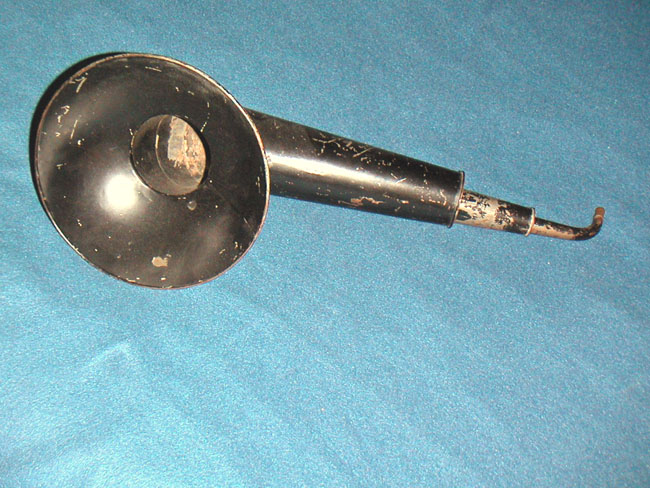
\includegraphics[width=0.25\textwidth]{trumpet}
    \caption{Trąbka słuchowa}
    \label{fig:trumpet}
\end{figure}
\end{frame}

\begin{frame}
\frametitle{Krótka historia II}
Pierwsze urządzenia eletroniczne do poprawy słuchu stworzono w XX wieku. Były one duże oraz ciężkię, więc trudne do noszenia.
\begin{figure}
    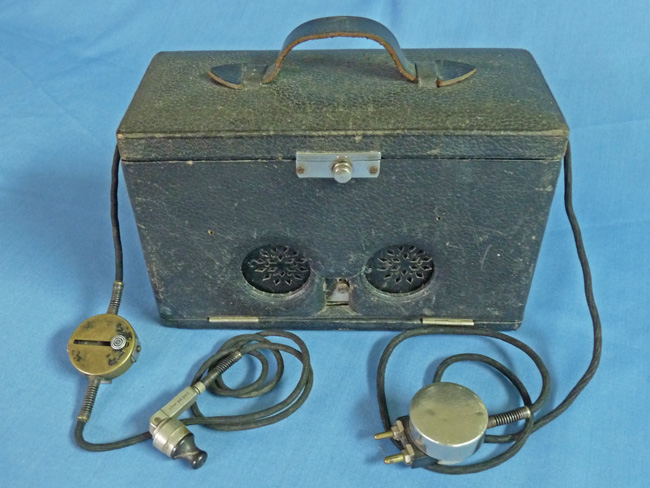
\includegraphics[width=0.3\textwidth]{siemens_old}
    \caption{Siemens/Fortiphone Model M-22 "Booster Flat" Carbon Hearing Aid}
    \label{fig:siemens-old}
\end{figure}
\end{frame}

\begin{frame}
W ciągu całego XX wieku ulepszano i pomniejszano aparaty. W tym momencie na rynku są dostępne aparaty, które łatwo ukryć wśród włosów oraz posiadające funkcje dodatakowe.
\frametitle{Krótka historia III}
\begin{figure}
    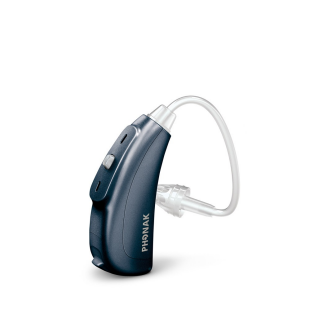
\includegraphics[width=0.25\textwidth]{phonak}
    \caption{Phonak Bolero Q}
    \label{fig:phonak}
\end{figure}
\end{frame}

\begin{frame}
\frametitle{Tłumienie szumu}
Większość obecnie dostępnych na rynku aparatów realizuje funkcję tłumienia szumu. Jest to pożądana funkcja dodatkowa, pozwalająca urządzeniu reagować podobnie jak ludzki słuch, który jest w stanie rejestrować tylko interesujące nas dźwięki. 

Dodatkową opcją, dostępną w mniejszej gamie modeli, jest redukcja szumu powstałego przez wiatr wiejący wokół mikrofonu. To jest również przydatna funkcja pozwalająca na lepsze działanie aparatu nie tylko w pomieszczeniach zamkniętych.
\end{frame}

\begin{frame}
\frametitle{Usuwanie sprzężeń zwrotnych}
Ta funkcja, podobnie jak tłumienie szumu, jest również bardzo pożądana w aparatach słuchowych. Także jest dostępna w większości oferowanych modeli.

Sprzężenia mogą się pojawić podczas normalnej pracy urządzenia i powodować dyskomfort oraz cheć zrezygnowania z aparatu. Dlatego to jest ważny dodatek.
\end{frame}

\begin{frame}
\frametitle{Tryb działania zależny od otoczenia}
Pozwala na zmianę parametrów aparatu w zależności od otoczenia. Zwiększa to komfort używania urządzenia, poprawia możliwości rozumienia słów. Jednak przy użyciu wcześniejszych funkcji nie jest niezbędna. Poprawne i wystarczające zrozumienie słów można osiągnąć bez jej obecności.

Ta funkcja jest dostępna w mniejszej ilości aparatów niż dwie poprzednie.
\end{frame}
%---------------------------------------------------------------------------



%---------------------------------------------------------------------------


\end{document}

